% My mini-preamble
\newcommand{\asgn}{\gets\,}
\newenvironment{landscape}{%
\newgeometry{textwidth=\textheight,textheight=\textwidth,left=15mm,top=15mm}%
\eject\pagewidth=297mm\pageheight=210mm%
}{%
\restoregeometry%
\eject\pagewidth=210mm\pageheight=297mm%
}

% The actual content begins here.
\section{Шейкерная сортировка. Сортировка Шелла}
Все сортировки в этом и следующем вопросах сортируют массив по возрастанию.
\subsection{Шейкерная сортировка}
Шейкерная сортировка относится к так называемым сортировкам обменом и представляет
собой усложненную версию пузырьковой сортировки, которая одновременно сортирует массив
в двух направлениях, перемещая большие числа к концу массива, а маленькие --- к его началу.
В среднем и в худшем случае сортировка имеет сложность $O(n^2)$. В лучшем случае, когда
массива уже отсортирован, алгоритм имеет сложность $O(n)$.

\begin{minted}{C++}
/// Сортирует массив в порядке возрастания
/// (за что этот алгоритм?)
void ShakerSort(int *a, int count) {
  if (count <= 1) {
    return;
  }
  // Нижняя и верхняя границы неотсортированного подмассива
  int left = 0;
  int right = count - 1;
  while (left != right) {
    int last_swap = left;
    // Поднятие больших чисел к концу массива
    for (int i = left; i < right; ++i) {
      if (a[i] > a[i + 1]) {
        std::swap(a[i], a[i + 1]);
        last_swap = i + 1;
      }
    }
    right = last_swap;
    // Перемещение маленьких чисел к началу массива
    for (int i = right; i > left; --i) {
      if (a[i] < a[i - 1]) {
        std::swap(a[i], a[i - 1]);
        last_swap = i - 1;
      }
    }
    left = last_swap;
  }
}  
\end{minted}

\subsection{Сортировка Шелла}
Сортировка Шелла является усовершенствованной версией сортировки вставками. Ее идея состоит
в том, чтобы перед тем, как сортировать весь массив, упорядочить некоторые элементы,
находящиеся на определенном расстоянии друг от друга.
\begin{figure}
  \begin{center}
  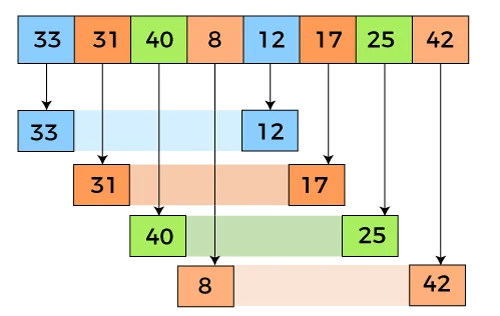
\includegraphics[scale=0.4]{27-34/shell-sort.png}
  \end{center}
  \caption{Сравнение элементов сортировкой Шелла, $h=n/2$.}
\end{figure}
Алгоритм сортирует массив в $k$ проходов. $i$-й проход характеризуется
значением смещения $h_i$ таким, что отдельно друг от друга сортируются подпоследоваетльности,
содержащие элементы, находящиеся на расстоянии
$h_i$ друг от друга. Шелл предлагал смещения $h_0 = \left\lfloor\tfrac{n}{2}\right\rfloor$,
$h_{i+1} = \left\lfloor\tfrac{h_i}{2}\right\rfloor$,
\dots, $h_{k-1} = 1$. Возможны и другие смещения, но всегда требуется, чтобы $h_{k-1} = 1$
и последовательность убывала.

На $i$-м шаге с помощью сортировки вставками между собой значения, в подпоследовательностях
вида $a_{i}^{(l)}[n] = a[l+ph_i]$, где $l$ задает номер подпоследовательности и индекс первого элемента
подпоследовательности в основном массиве, а номер $p$ изменяется в таких пределах,
чтобы элементы списка $a_{i}^{(l)}$ прошли наибольшее число элементов массива $a$,
не выходя за его пределы. Затем отсортированные списки объединяются в массив,
после чего массив вновь разбивается на списки, но уже со смещением $h_{i+1}$.
Данные действия повторяются ровно $k$ раз.

Сложность алгоритма сортировки Шелла зависит от выбора смещений на каждом шаге.
Ниже приведена сводная таблица некоторых схем.
\begin{longtable}{p{2cm}p{8cm}l}
  Автор   & Схема & Сложность \\ \hline
  Шелл    & см. выше & $O(n^2)$ \\
  Хиббард & \begin{minipage}{5cm} Все значения\\ $2^i - 1 \leq n\,\, \forall i \in \mathbb{N}$ \end{minipage} &  $O(n^{\frac 3 2})$ \\
  % FIXME: powers
  Седжвик & $h_i = \begin{cases}
    9\cdot 2^i - 9\cdot 2^{i/2} + 1, 2 \mid (i+1) \\
    8\cdot 2^i - 6\cdot 2^{(i+1)/2} + 1, 2 \not\mid (i+1)
  \end{cases}$ & $O(n^{\frac 7 6})$..$O(n^{\frac 4 3})$ \\
  Пратт   & \begin{minipage}{5cm} Все значения \\ $2^i \cdot 3^j \leq n/2\,\, \forall i,j \in \mathbb{N}$ \end{minipage} & $O(n\log^2 n)$ \\ \hline
\end{longtable}

\begin{minted}{C++}
/// Сортирует массив array размера size с помощью сортировки Шелла,
/// использующей схему Шелла
void ShellSort(int *array, int size) {
    for (int s = size / 2; s > 0; s /= 2) {
        for (int i = s; i < size; ++i) {
            for (int j = i - s; j >= 0 && array[j] > array[j + s]; j -= s) {
                std::swap(array[j], array[j+s]);
            }
        }
    }
}
\end{minted}

\section{Сортировка Хоара – алгоритм QuickSort. Сортировка слиянием}
\subsection{QuickSort (быстрая сортировка)}
Time Complexity --- $O(n\log n)$ в среднем, $O(n^2)$
в худшем (если входной массив отсортирован в обратном порядке) случае.
Space Complexity зависит от функции разбиения (функция Хоара дает $\log n$ на стек рекурсивных вызовов).

Быстрая сортировка функционирует по принципу <<разделяй и властвуй>>.
Пусть требуется отсортировать массив из $n$ элементов $a[1\dots n]$ (обе границы включены).
На первом шаге полагаем $l=1$ и $r=n$. Далее придерживаемся следующего алгоритма:
\begin{enumerate}
  \item Вычислить индекс $q$ опорного элемента.
  \item Массив $a[l\dots r]$
  разбивается на два подмассива $a[l\dots q]$ и $a[q+1\dots r]$, таких что каждый элемент $a[l\dots q]$
  меньше или равен $a[q]$, который в свою очередь, не превышает любой элемент подмассива $a[q+1\dots r]$, то есть
  \begin{align*}
    \forall\, n <&q \quad a[n] \leq a[q] \\
    \forall\, m >&q \quad a[q] \leq a[m].
  \end{align*}
  \item Подмассивы $a[l\dots q]$ и $a[q+1\dots r]$ сортируются рекурсивно.
\end{enumerate}

Распространенной является функция разбиения Хоара, которая выбирает медианный элемент массива
в качестве опорного.

Отметим, что в качестве опорного можно выбирать абсолютно любой элемент массива
(даже всегда первый, но при такой реализации сложность любого случая будет $\Theta(n^2)$).

Если кому-либо известен алгоритм функции разбиения, то он может злонамеренно соорудить
такой массив, на котором функция быстрой сортировки уйдет в $O(n^2)$ и/или возникнет
переполнение стека. Чтобы избежать этого, в качестве опорного можно выбирать случайный
элемент массива.

Ниже приведен алгоритм Quicksort с разбиением Хоара.
\begin{minted}{C++}
/// a - массив, который сортируется
/// l - левая граница сортируемого отрезка
/// r - правая граница
int Partition(int *a, int l, int r) {
  int v = a[(l + r) / 2];
  int i = l;
  int j = r;
  while (i <= j) {
    while (a[i] < v) {
      ++i;
    }
    while (a[j] > v) {
      --j;
    }
    if (i >= j) {
      break;
    }
    std::swap(a[i++], a[j--]);
  }
  return j;
}

void Quicksort(int *a, int l, int r) {
  if (l < r) {
    int q = Partition(a, l, r);
    Quicksort(a, l, q);
    Quicksort(a, q + 1, r);
  }
}
\end{minted}

\subsection{Сортировка слиянием}
Данный алгоритм также использует стратегию <<разделяй и властвуй>>, рекурсивно сортируя
поданный на вход массив следующим образом:
\begin{enumerate}
  \item Массив разделяется на два подмассива так, чтобы их длины отличались не больше,
        чем на единицу;
  \item Каждый из подмассивов сортируется по отдельности рекурсивным вызовом;
  \item Посортированные массивы объединяются в один. Первый элемент результирующего 
        массива равен наименьшему из элементов подмассивов и так далее.
\end{enumerate}

Нетрудно заметить, что такая реализация потребует $O(n)$ дополнительной памяти.
Существует реализация сортировки слиянием, которая не требует дополнительной памяти,
однако она имеет большую временную сложность: $O(\log^2 n)$ против $O(\log n)$.
Ниже приведена реализация обычного алгоритма сортировки слиянием. Здесь используются
два массива, которые поочередно меняются местами. В каждом из этих массивов
в данный момент времени сортируется только одна половина исходного массива.

\begin{minted}{C++}
int *MergesortImpl(int *up, int *down, int left, int right) {
  if (left == right) {
    down[left] = up[left];
    return down;
  }

  unsigned int middle = left + (right - left) / 2;

  int *l_buff = MergesortImpl(up, down, left, middle);
  int *r_buff = MergesortImpl(up, down, middle + 1, right);

  int *target = l_buff == up ? down : up;

  unsigned int l_cur = left, r_cur = middle + 1;
  for (unsigned int i = left; i <= right; i++) {
    if (l_cur <= middle && r_cur <= right) {
      if (l_buff[l_cur] < r_buff[r_cur]) {
        target[i] = l_buff[l_cur];
        l_cur++;
      } else {
        target[i] = r_buff[r_cur];
        r_cur++;
      }
    } else if (l_cur <= middle) {
      target[i] = l_buff[l_cur];
      l_cur++;
    } else {
      target[i] = r_buff[r_cur];
      r_cur++;
    }
  }
  return target;
}

void Mergesort(int *array, int len) {
  int *back = new int[len];
  std::copy(array, array + len, back);
  int *sorted = MergesortImpl(array, back, 0, len - 1);
  if (sorted != array) {
    std::copy(back, back + len, array);
  }
  delete[] back;
}
\end{minted}

\section{Бинарные деревья – основные понятия. Основные операции с бинарными деревьями}
Через $n$ будем обозначать общее число узлов в дереве.
\subsection{Определения}
\textbf{Дерево} --- связный ациклический иерархически построенный граф. Граф обычно
полагается ориентированным в направлении иерархии: в каждую вершину (кроме одной,
называемой \textbf{корнем}) входит ровно одно ребро, но исходить из вершины может
произвольное количество ребер. Каждой вершине при этом сопоставляются какие-либо данные.

\textbf{Бинарным (двоичным) деревом} называется такое дерево, из каждой вершины которого
исходит не более двух ребер.

Особый интерес представляют бинарные деревья поиска и кучи.

Когда речь идет о структурах данных, вершины принято называть \textbf{узлами}.
Данные, находящиеся в конкретном узле называют его \textbf{ключом}, а если дерево задает
отображение, то к ключам также добавляется \textbf{значения}.

\textbf{Ветвь} дерева --- дуга, соединяющая два узла. 

\textbf{Лист (терминальный узел)} --- узел, не имеющий исходящих ветвей.

\textbf{Внутренний узел} --- узел, имеющий как входящие, так и исходящие ветви.

Каждая ветвь задает пару \textbf{родителя} --- узла, из которого данная ветвь исходит
и \textbf{потомка} --- узла, в который данная ветвь входит. Потомками также называют
потомков потомков.

\textbf{Поддеревом} дерева называется некоторый узел вместе со всеми своими потомками.

\textbf{Глубина (уровень)} узла --- расстояние от узла до корня.

\textbf{Высота} узла --- максимальное расстояние от узла до листа. Высота дерева считается
равной высоте его корня.

\textbf{Бинарной кучей} называется бинарное дерево, для которого выполнено следующее:
\begin{enumerate}
  \item Значение в каждой вершине не больше (не меньше), чем в ее потомках;
  \item Дерево сбалансировано;
  \item Последний слой заполнен слева направо без дырок.
\end{enumerate}
Кучи подробнее рассмотрены в \ref{sec:heap}.

\phantomsection
\label{def:bst}
Бинарное дерево называется бинарным \textbf{деревом поиска}, если для любого его узла выполнено:
\begin{enumerate}
  \item Ключи левого ребенка и всех его потомков не превосходит ключ данного узла;
  \item Ключ данного узла не превосходит ключей его правого ребенка и всех потомков последнего.
\end{enumerate}
В случае несуществования у узла какого-либо ребенка в данном определении следует опустить соответствующее условие.

{\small\itshape Замечание. В данных условиях можно одновременно заменить знак неравенства на противоположный.}

К основным операциям на бинарных деревьях поиска относятся добавление, удаление и поиск узла (см. вопрос \ref{sec:tree-node-ops}),
поиск минимума и максимума, а также обход дерева.

\subsection{Обход}
\textbf{Обход дерева} --- посещение всех узлов дерева в определенном порядке и обработка содержащихся в них данных.
Выделяют четыре основных порядка обхода: в ширину, в прямом порядке, в обратном порядке и в симметричном порядке.
Алгоритм обхода в ширину использует $O(n)$ дополнительной памяти, остальные алгоритмы используют $O(\log n)$ памяти
на \textit{стек вызовов} {\color{red} TODO: ссылка на вопрос про стек вызовов}.

Предположим, что мы имеем дело с бинарным деревом поиска. Тогда обход в прямом порядке будет обрабатывать значения
в порядке их возрастания. Ниже приведен алгоритм обхода в прямом порядке на псевдокоде.
\begin{algorithmic}
  \Function{PreOrder}{Node n}
    \State Handle n
    \Comment{Обработать n}
    \If{n has left child}
      \State \Call{PreOrder}{n.left}
      \Comment{Посетить левое поддерево}
    \EndIf
    \If{n has right child}
      \State \Call{PreOrder}{n.right}
      \Comment{Посетить правое поддерево}
    \EndIf
  \EndFunction
\end{algorithmic}

Алгоритм обхода в обратном порядке:
\begin{algorithmic}
  \Function{PostOrder}{Node n}
    \If {n has left child}
      \State \Call{PostOrder}{n.left}
    \EndIf
    \If{n has right child}
      \State \Call{PostOrder}{n.right}
    \EndIf
    \State Handle n
  \EndFunction
\end{algorithmic}

Алгоритм симметричного обхода:
\begin{algorithmic}
  \Function{InOrder}{Node n}
    \If {n has left child}
      \State \Call{InOrder}{n.left}
    \EndIf
    \State Handle n
    \If{n has right child}
      \State \Call{InOrder}{n.right}
    \EndIf
  \EndFunction
\end{algorithmic}

Алгоритм обхода дерева в ширину посещает дерево слой за слоем: сначала посещается корневой узел,
затем его дети (все вершины глубины 1), после них алгоритм посещает все вершины глубины 2 и так
далее, пока не будут исчерпаны все вершины.
\begin{algorithmic}[1]
  \Function{Bfs}{Node n}
    \State q $\gets$ empty Queue
    \State \Call{q.Push}{n}
    \While{q is not empty}
      \State m $\gets$ q.\Call{Pop}{}
      \State Handle m
      \If {n has left child}
        \State q.\Call{Push}{n.left}
      \EndIf
      \If{n has right child}
        \State q.\Call{Push}{n.right}
      \EndIf
    \EndWhile
  \EndFunction
\end{algorithmic}

\subsection{Поиск минимума (максимума)}
Минимальным элементом дерева является его самый левый элемент, а максимальным --- самый правый.
\begin{minted}{C++}
Node* MinNode(Node* root) {
  while (root->left != nullptr) {
    root = root->left;
  }
  return root;
}
Node* MaxNode(Node* root) {
  while (root->right != nullptr) {
    root = root->right;
  }
  return root;
}
\end{minted}

Для бинарных поисковых деревьев вводятся \hyperref[sec:tree-node-ops]{алгоритмы добавления, поиска и удаления элементов}.

Для самобалансирующихся деревьев дополнительно вводятся \hyperref[sec:rotations]{алгоритмы поворотов}.

\section{Понятие рекурсивного типа данных}
\textbf{Рекурсивным типом данных} является всякий тип данных, который в своем объявлении содержит ссылается
на себя. Иными словами, он содержит поле, которое имеет тип ссылки или указателя на этот же тип данных.

С помощью рекурсивных типов реализуются узлы таких структур данных, как списки и деревья, которые
содержат ссылки на потомков и предков. Рекурсивные типы позволяют описывать потенциально бесконечные
последовательности. Их использование удобно при обработке иерархических типов данных.

В языке \verb|C++| структура (класс, объединение) не является полным типом до конца
своего объявления, и посему не может содержать саму себя в качестве поля. Действительно, если бы структура
могла содержать саму себя, то она бы имела бесконечный размер, который невозможно поместить в конечную память.

При этом структура принципиально может содержать указатель или ссылку на себя. Если структура содержит ссылку на себя
в качестве поля, то эта ссылка должна быть проинициализирована при создании объекта структуры. Объект структуры со
ссылкой на себя не может быть впервые создан с помощью какого-либо конструктора, и потому без черной магии его
создать невозможно.

Структуру, содержащую указатель на себя, возможно создать не прибегая к каким-либо ухищрениям,
и потому мы будем рассматривать только их.

\begin{minted}{C++}
// Узел дерева. Содержит указатель на родителя и двух потомков.
template<typename T>
struct TreeNode {
  T data;
  TreeNode *parent = nullptr;
  TreeNode *left = nullptr;
  TreeNode *right = nullptr;
}
// Узел двусвязного списка. Содержит указатель на предыдущий и следующий узел.
template<typename T>
struct DoubleLinkedListNode {
  T data;
  DoubleLinkedListNode* prev = nullptr;
  DoubleLinkedListNode* next = nullptr;
}
// Узел односвязного списка. Содержит указатель на следующий узел.
template<typename T>
struct ForwardListNode {
  T data;
  ForwardListNode *next = nullptr;
}
\end{minted}

\section{Поиск и включение для деревьев. Исключение для деревьев}
\label{sec:tree-node-ops}
Рассмотрим операции над \hyperref[def:bst]{бинарными деревьями поиска} (BST) в их наивной реализации.
У самобалансирующихся деревьев операции вставки и удаления будут устроены более сложно, однако
операция поиска останется такой же.

Все описанные здесь операции имеют вычислительную сложность $O(\log n)$ в лучшем
и $O(n)$ в худшем случае.

\subsection{Поиск}
Поиск в BST по своей сути напоминает бинарный поиск в линейном массиве.
Если значение в текущем узле совпадает с целевым, то мы возвращаем этот узел.
Если значение в текущем узле меньше целевого, то мы запускаем поиск в левом поддереве.
В противном случае поиск запускается в правом поддереве.
\begin{minted}{C++}
Node* Find(Node* root, int value) {
  while (root != nullptr && root->data != value) {
    if (value < root->data) {
      root = root->left;
    } else {
      root = root->right;
    }
  }
  return n;
}
\end{minted}
\subsection{Вставка (<<включение>>)}
Вставка работает аналогично поиску, однако при обнаружении у элемента отсутствия ребенка
нужно подвесить на него вставляемый элемент.
\begin{minted}{C++}
Node* Insert(Node* root, int value) {
  while (root != nullptr) {
    if (value < root->data) {
      if (root->left != nullptr) {
        root = root->left;
      } else {
        root->left = new Node(value);
        root->left->parent = root;
        return root->left;
      }
    } else if (root->data < value) {
      if (root->right != nullptr) {
        root = root->right;
      } else {
        root->right = new Node(value);
        root->right->parent = root;
        return root->right;
      }
    } else {
      // Value already exists in the tree
      return root;
    }
  }
  return n;
}
\end{minted}
\subsection{Удаление (<<Исключение>>)}
Для удаления узла с заданным значением его сперва надо найти. Затем мы столкнемся с одним из трех случаев:
\begin{enumerate}
  \itembf{Узел имеет двух детей.} Данный узел заменяется наибольшим узлом в левом поддереве либо наименьшим узлом в правом, после чего удаляется.
  \itembf{Узел листовой.} Он просто удаляется, ссылка родителя на этот узел устанавливается в \mverb{nullptr}.
  \itembf{Узел имеет одного ребенка.} Вместо данного узла к его родителю подвешивается единственный ребенок. Данный узел удаляется.
\end{enumerate}
% Алгоритм какой-то громоздкий, поэтому пока что его опустим.
% https://neerc.ifmo.ru/wiki/index.php?title=Дерево_поиска,_наивная_реализация
% \begin{minted}{C++}
% bool IsLeftChild(Node* child) {
%   return child->parent->left == child;
% }
% void Delete(Node* root, int value) {
%   while (root != nullptr) {
%     Node* n = Find(root, value);
%     if (n == nullptr) {
%       // No such value
%       return;
%     }
%     // Здесь не обработан краевой случай n->parent == nullptr,
%     // поскольку он внесет излишнюю громоздкость
%     // Случай 1: оба ребенка
%     if (n->left != nullptr && n->right != nullptr) {
%       Node* m = MinNode(n->right);
%       if (IsLeftChild(m)) {

%       }
%     } else if (n->left == nullptr && n->right == nullptr) {
%       if (IsLeftChild(n)) {
%         n->parent->left = nullptr;
%         delete n;
%       } else {
%         n->parent->right = nullptr;
%         delete n;
%       }
%     } // Случай 3: один ребенок
%     else if (n->left != nullptr) {
%       n->parent->
%     }
%   }
%   return n;
% }
% \end{minted}

\section{Сбалансированные деревья. Сортировка с помощью бинарных деревьев (кучи)}
Дерево называется \textbf{сбалансированным}, если максимальное значения модуля разности глубин
любых двух его листов не превышает единицы.

На сбалансированных деревьев алгоритмы поиска, вставки и удаления не деградируют до $O(n)$
и всегда имеют сложность $O(\log n)$.

Для балансировки деревьев можно использовать несколько подходов.
\subsection{Ручная балансировка}
Самые неэффективный и наивный подход к балансировке. Дерево разворачивается
в линейную отсортированную структуру и собирается заново в уже сбалансированном варианте
(корнем выбирается медиана списка/массива, его детьми --- медианы половин и так далее).
Имеет сложность $O(n^2)$ при использовании списка и $O(n\log n)$ --- массива.

Более эффективное способом поддержания сбалансированности дерева является использование
самобалансирующихся структур, в основе которых лежат следующие подходы
\begin{itemize}
  \item Нарушение баланса при добавлении (удалении) узла возникают только на пути от корня к данному узлу,
  не затрагивая остальные поддеревья;
  \item Перенос узла внутри дерева осуществляется быстрее, чем его полная размотка и сборка.
\end{itemize}

Распространенными самобалансирующимися деревьями являются красно-черные и АВЛ-деревья.

\subsection{Повороты}
\label{sec:rotations}
Как в красно-черных, так и в АВЛ-деревьях для восстановления баланса используются
\textbf{повороты} --- специальные преобразования структуры дерева.

Разделяют четыре вида поворотов, которые получаются в результате декартова произведения двух признаков:
большие и малые, левые и правые повороты. Правые повороты проводятся симметрично левым, поэтому рассмотрим
только левые.

% TODO: check left and right
В левом малом повороте (рис.~\ref{fig:small-rotation}) корень ($a$) и его правый потомок ($b$)
меняются местами, а левое поддерево ($Q$) нового корня $b$ становится правым потомком старого корня $a$.

В правом малом повороте (рис.~\ref{fig:small-rotation}) корень ($a$) и его левый потомок ($b$)
меняются местами, а правое поддерево ($Q$) нового корня $b$ становится левым потомком старого корня $a$.

Большие повороты являются комбинациями малых. Для левого поворота сперва осуществляется правый поворот
правого ребенка корная, а затем --- левый поворот самого корня (см. рис. \ref{fig:big-rotation}).

\begin{figure}
  \begin{center}
  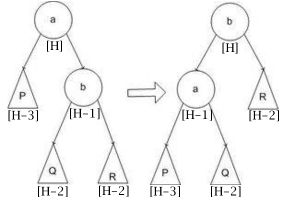
\includegraphics{27-34/small-rotation.jpg}
  \caption{Малый левый поворот}
  \label{fig:small-rotation}
  \end{center}
\end{figure}
\begin{figure}
  \begin{center}
  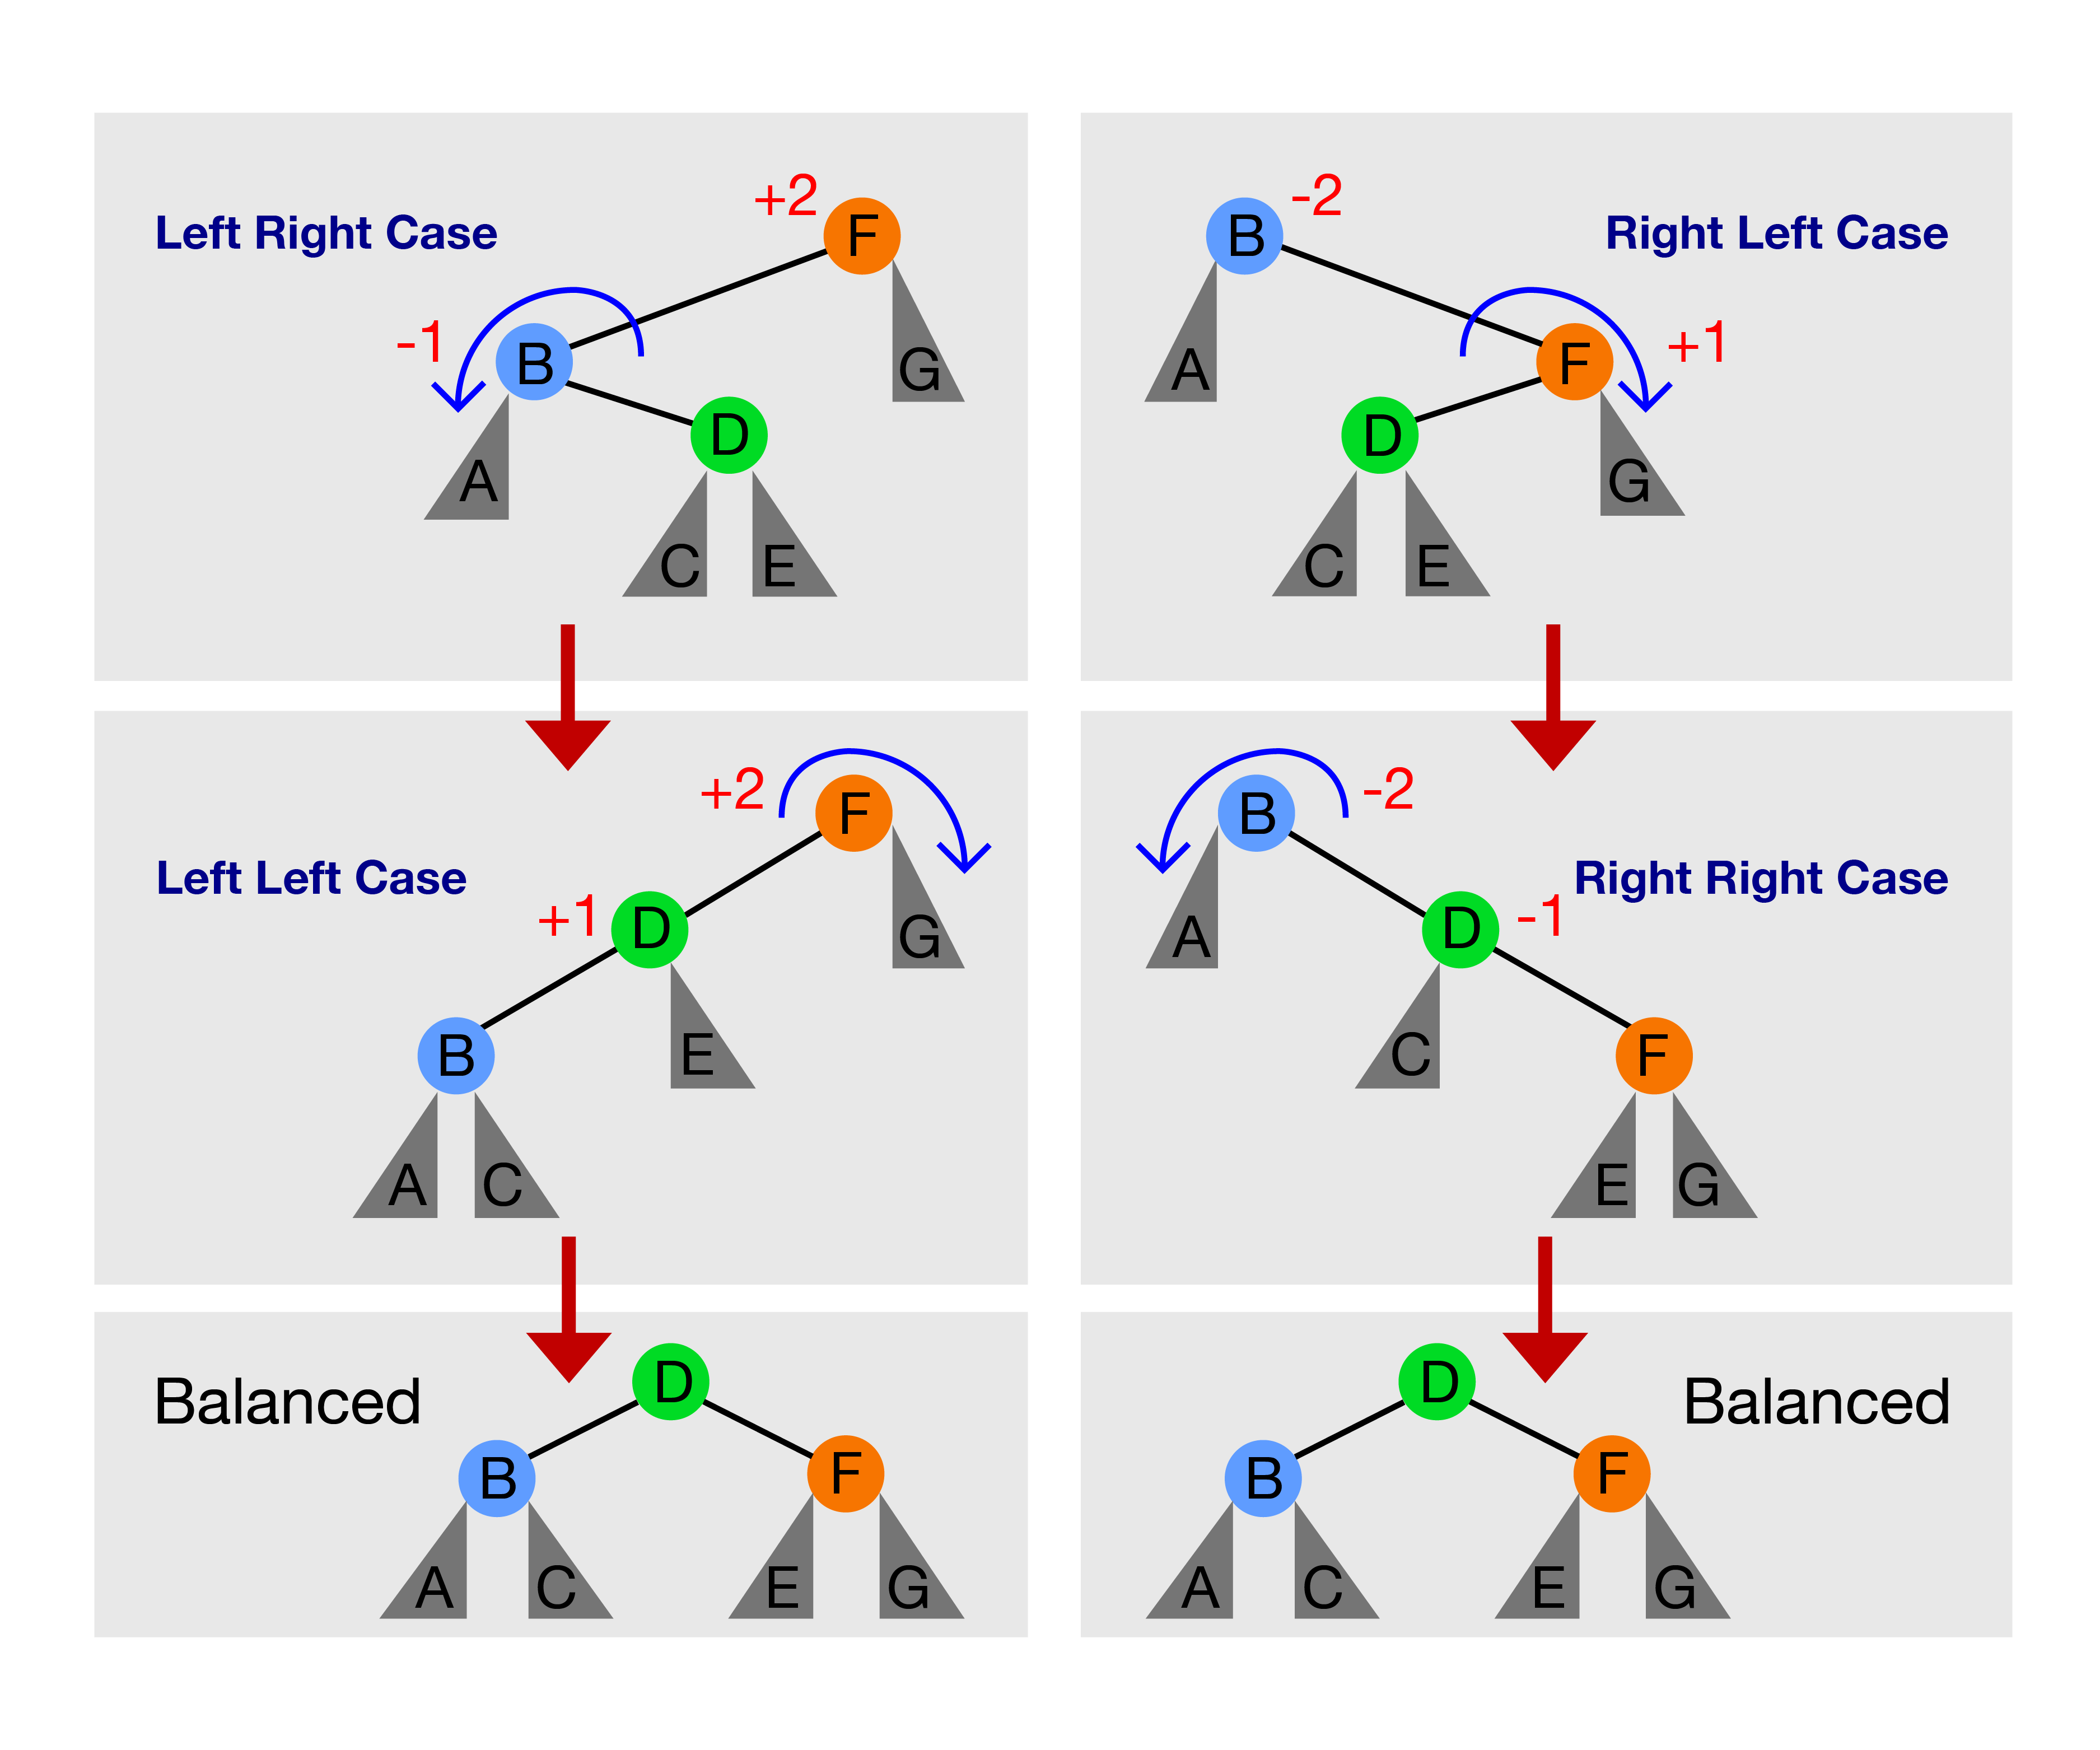
\includegraphics[scale=0.14]{27-34/both-big-rotations.png}
  \caption{Большие \textit{правый} и \textit{левый} повороты (именно в таком порядке!)}
  \label{fig:big-rotation}
  \end{center}
\end{figure}

\subsection{Красно-черное дерево}
В красно-черном дереве (КЧД) для узлов вводится дополнительная характеристика --- цвет.
Правильно построенное КЧД поддерживает следующие инварианты:
\begin{enumerate}
  \item Терминальные узлы фиктивные и не содержат данных;
  \item Корневой и терминальные узлы черные;
  \item У красного узла оба ребенка черные;
  \item Каждый путь от заданного узла до его листового потомка содержит одинаковое количество черных узлов.
\end{enumerate}

Общий алгоритм добавления узла в КЧД таков:
\begin{algorithmic}
  \Procedure{AddNode}{RBTree $t$, Value $v$}
    \State Find a leaf node $u$ to substitute with a new node
    \State $u$ \asgn new Node($v$)
    \State Set $u$'s children to BLACK NIL nodes
    \State $u$.color \asgn RED
    \If{invariant is broken}
      \State $u$.color \asgn BLACK
      \State Fix invariant via rotations
    \EndIf
  \EndProcedure
\end{algorithmic}
\subsection{АВЛ-дерево}
Для каждого узла АВЛ-дерева определяется \textbf{показатель баланса} --- разность
высоты левого и правого поддеревьев данного узла.

Дерево считается сбалансированным, если в каждой его вершине показатель баланса
по модулю не превосходит единицы. АВЛ-деревья сбалансированы не идеально, но близко
к тому и гораздо лучше, чем КЧД.

При удалении или вставке нового узла происходит пересчет балансов у всех вершин дерева на пути к корню
и его восстановление с помощью поворотов.

\subsection{Саморегулирующееся дерево}
Примером саморегулирующихся деревьев является Splay-дерево, которое поддерживает баланс в среднем.
Амортизированная сложность операций поиска, вставки и удаления равна $O(\log n)$. Дерево не хранит
в своих вершинах каких-либо дополнительных данных. При доступе к вершине дерева она продвигается в корень.

\subsection{Сортировка кучей (HeapSort)}
\label{sec:heap}

Бинарную кучу в памяти принято представлять в виде массива $a$ длины $n$.
Левым ребенком узла с индексом $i$ считается узел с индексом $2i+1$,
правым --- с индексом $2i+2$. Для сортировки по возрастанию мы будем рассматривать кучу
на максимумы. Для нее по определению выполняется:
$$ a[i] \geq a[2i+1]\, \land\, a[i] \geq a[2i+2]. $$

{\small
\textit{Примечание.} Для кучи определены основные операции:
\begin{enumerate}
  \item Извлечение максимального элемента;
  \item Добавление произвольного элемента;
  \item Уменьшение и увеличение произвольного элемента.
\end{enumerate}
}

Сортировка кучей (пирамидальная сортировка) предполагает использование свойства кучи для упорядочения массива:
сперва из массива делается куча, затем, пока в куче не останется только один элемент,
из нее извлекается максимальный элемент и отправляется в конец части массива $a$,
занятой кучей (вначале она совпадает со всем массивом), а затем длина части массива,
занятой кучей, уменьшается на единицу. Таким образом, массив всегда как бы разделяется
надвое: в одной части находится неотсортированная куча, а в конце --- отсортированный
подмассив.

HeapSort имеет сложность $O(n\log n)$ для каждого случая и не требует дополнительной памяти. В некоторых
реализациях сортировки этот алгоритм используется вместе с быстрой сортировкой для случаев, когда
последняя уходит в слишком глубокую рекурсию.

\begin{minted}{C++}
// Опускает элемент с индексом i вниз до тех пор,
// пока не восстановится свойство кучи.
void SiftDown(int *heap, int len, int i) {
  while (2 * i + 1 < len) {
    int left = 2 * i + 1;
    int right = 2 * i + 2;
    int j = left;
    if (right < len && heap[right] > heap[left]) {
      j = right;
    }
    if (heap[i] >= heap[j]) {
      break;
    }
    std::swap(heap[i], heap[j]);
    i = j;
  }
}

/// Переставляет элементы массива heap так, чтобы он стал кучей.
void Heapify(int *heap, int len) {
  for (int i = len / 2; i >= 0; --i) {
    if (2 * i + 1 < len && heap[i] <= heap[2 * i + 1]) {
      SiftDown(heap, len, i);
    }
  }
}

/// Сортирует кучей массив array длины len.
void Heapsort(int *array, int len) {
  // Сделать массив кучей
  Heapify(array, len);
  // Длина части массива, в которой содержится куча
  int remaining = len;
  for (int i = 0; i < len - 1; ++i) {
    // Поменять местами первый и последний элемент кучи
    // (len - i - 1 == remaining?)
    std::swap(array[0], array[len - i - 1]);
    --remaining;
    // Восстановить свойство кучи
    SiftDown(array, remaining, 0);
  }
}
\end{minted}
\section{Графы и возможные формы их описания. Нахождение кратчайшего пути на графе}
В этом и следующем разделе для число вершин графа обозначается через $V$, а число ребер~--- через $E$.
Графы в программировании представляют собой обобщение деревьев и подобны графам из математики.
Каждой вершине графа сопоставляется какое-либо значение, а некоторые пары вершин соединены
ребрами.

\subsection{Способы представления}
Способы задания графов в памяти компьютера в целом такие же, как и в математике,
за исключением того, что иногда матрицы заменяют списками для оптимизации
пространственной сложности. Отметим, что сами вершины обычно хранятся в виде
массива, в то время как для представления топологии доступны разнообразные структуры.

% TODO: Arrange the figures somehow.
\begin{figure}[H]
\begin{center}
  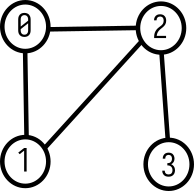
\includegraphics[scale=0.4]{27-34/sample-graph3.png}
  \caption{Граф с нумерованными (индексированными) вершинами}
  \label{fig:graph}
\end{center}
\end{figure}
\begin{figure}[H]
\begin{center}
  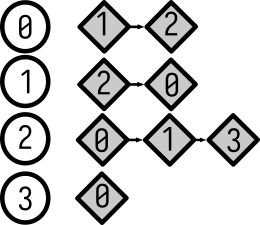
\includegraphics[scale=0.6]{27-34/adjacency-list.png}
  \caption{Список смежности}
  \label{fig:adj-list}
\end{center}
\end{figure}[H]
\begin{figure}
  {\large $$ \begin{array}{c|c}
      & \begin{matrix} 0 & 1 & 2 & 3 \end{matrix} \\\hline
    0 & \begin{matrix} 0 & 1 & 1 & 0 \end{matrix} \\
    1 & \begin{matrix} 1 & 0 & 1 & 0 \end{matrix} \\
    2 & \begin{matrix} 1 & 1 & 0 & 1 \end{matrix} \\
    3 & \begin{matrix} 0 & 0 & 1 & 0 \end{matrix} \\
  \end{array} $$}
  \caption{Матрица смежности}
  \label{fig:adj-mat}
\end{figure}
\begin{figure}
  \begin{center}
    $$[0, 1]\rightarrow[1, 2]\rightarrow[0, 1]\rightarrow[2, 3]$$
  \end{center}
  \caption{Список ребер}
  \label{fig:edg-list}
\end{figure}


\begin{minipage}{16cm}
\begin{longtable}[]{@{}>{\raggedright}p{3cm}p{100mm}p{3cm}@{}}
  Тип представления & Описание & Занимаемое место \\ \hline
  Матрица смежности &
    Данные, соответствующие узлам графа хранятся в виде одномерного массива \verb|b|.
    Дуги графа хранятся в виде двумерного булева массива (матрицы смежности) \verb|a[i][j]|,
    причем \mverb{a[i][j] == true} тогда и только тогда, когда вершины \verb|b[i]| и \verb|b[j]|
    соединены дугой. Для неориентированных графов необходимо дублировать записи в матрице смежности,
    чтобы она была симметричной.
  & $O(E+V^2)$ \\ \hline

  Список (массив) смежности &
    Для каждой вершины хранится список (или массив) индексов смежных с ней вершин. Очень
    похоже на предыдущий пункт за исключением того, для отсутствующих ребер ничего не хранится.
  & O(V+E) \\ \hline

  Список ребер &
    Граф представляется в виде списка или массива пар индексов смежных вершин.
    Для представления неориентированного графа для каждой пары смежных вершин $a$ и $b$
    хранят два ребра: $[a, b]$ и $[b, a]$.
  & O(E) \\ \hline

  Структура с оглавлением &
    Данное представление получается из массивов смежности путем их объединения
    в один большой массив. Для каждой вершины дополнительно хранится индекс, с которого начинается
    ее массив смежности в объединенном массиве. Он заканчивается на индексе,
    который находится перед индексом следующей вершины.
  & O(V+E) \\ \hline
  \caption{Некоторые способы представления графов в памяти}
\end{longtable}
\end{minipage}

\subsection{Поиск кратчайшего пути}
Задача поиска кратчайшего пути отдельно рассматривается для взвешенных
и невзвешенных графов. Напомним, у взвешенных графов графов каждому
ребру поставлено в соответствие какое-либо число --- вес ребра, или длина
пути. Задача поиска кратчайшего пути на взвешенных графах сводится к поиску
такого пути от одной вершины к другой, что сумма весов ребер на этом пути минимальна.
Кратчайший путь на невзвешенных графах представляет собой такой путь, в котором
меньше всего ребер.

\subsubsection{BFS для невзвешенных графов}
Для поиска пути на невзвешенных графов используется поиска в ширину. Ниже приведен псевдокод функции,
осуществляющей поиск кратчайшего пути в невзвешенном графе. Данная функция возвращает перечень вершин,
через которые надо пройти, чтобы попасть из узла $origin$ в узел $destination$, включающий эти узы.
\begin{algorithmic}
\Function{BfsPathFind}{Graph $g$, NodeIndex $origin$, NodeIndex $destination$}
\LComment{Здесь NodeIndex --- это тип индекса вершины графа.}
  \State $q$ \asgn empty Queue
  \State $visited$ \asgn empty Container
  \State $path$ \asgn empty Container
  \State $comefrom$ \asgn Array of length $g.V$
  \State $q$.\Call{Push}{$origin$}
  \While{$q$ is not empty}
    \State $n$ \asgn $q$.\Call{Pop}{}
    \State $visited$.\Call{Add}{$n$.index}
    \If{$n$ = $destination$}
      \State $visited$.\Call{Append}{$destination$}
      \While{$n \neq origin$}
        \State $n \gets visited[n]$
        \State $visited$.\Call{Append}{$n$}
      \EndWhile
      \State \Return{$path$.\Call{Reverse}{}}
    \EndIf
    \ForAll{adjacent nodes $m$ of $n$}
      \If{$m.\text{index} \notin visited$}
        \State $comefrom[m.\text{index}] \gets n$
        \State $q$.\Call{Push}{m.index}
      \EndIf
    \EndFor
  \EndWhile
  \State \Return{$path$} \Comment{Пустой путь}
\EndFunction
\end{algorithmic}

\subsection{Взвешенные графы}
Для поиска кратчайшего пути на взвешенных графах можно использовать алгоритмы из
\hyperref[sec:dijkstra_ford]{следующего вопроса}.

\section{Алгоритм Дейкстры, алгоритм Форда\footnote{Я полагаю, из всех алгоритмов,
носящих светлое имя Лестера Форда, здесь имеется в виду алгоритм Беллмана-Форда.}}
\phantomsection
\label{sec:dijkstra_ford}
Алгоритм Дейкстры и алгоритм Форда предназначены
для поиска кратчайшего пути во взвешенном графе.
Обычно алгоритм Дейкстры является более эффективным, однако он,
в отличие от алгоритма Беллмана-Форда, не поддерживает отрицательные
веса на ребрах. Оба алгоритма в результате своей работы позволяют проставить
расстояния от стартовой вершины до всех вершин графа.

Ниже приведены
реализации алгоритмов, которые лишь расставляют длины путей.
Чтобы получить сам путь, необходимо предварительно завести массив $p$ длины $V$.
Пусть при раскрытии вершины с индексом $v$ обновилась длина пути от начальной вершины $s$ до вершины
с индексом $u$. Тогда надо дополнительно произвести присваивание $p[v] \gets u$.
Путь из начальной вершины до вершины $u$ восстанавливается следующим образом:
$$u \gets p[u] \gets p[p[u]] \gets \cdots \gets p[p[\dots p[u]]] = s. $$

\subsection{Алгоритм Дейкстры}
Алгоритм Дейкстры поддерживает массив расстояний от данной вершины до всех
остальных вершин графа и перечень индексов необработанных вершин, который хранится в
виде приоритетной очереди (кучи), упорядоченной по возрастанию пути от данной вершины.
Перед началом работы алгоритма расстояние до начальной вершины устанавливается в нуль,
а остальные расстояния --- в бесконечность.

На каждом шаге алгоритма из очереди с необработанными вершинами извлекается
вершина, ближайшая к данной. Затем для каждого соседа извлеченной вершины
обновляется расстояние: если сумма расстояний от начальной вершины до извлеченной
и от извлеченной вершины Ко соседа меньше, чем текущее значение длины пути от начальной
вершины до соседа, то оно уменьшается.

Алгоритм повторяется до тех пор, пока не будет извлечена целевая вершина.
Если очередь была исчерпана, а целевая вершина из нее не была извлечена, то
граф не является связным и пути между данными вершинами не существует.

\begin{minted}{C++}
// Реализация с Википедии
#include <bits/stdc++.h>

typedef long long ll;

int main() {
  ll inf = LLONG_MAX;
  int n, m, a, b;
  ll c;
  std::cin >> n >> m; // n - кол-во вершин; m - кол-во рёбер
  // Граф представляется в виде массива смежности
  std::vector<std::vector<std::pair<int, ll>>> country(
      n); // в country[v] хранится пара (u, c), это означает, что из v есть
          // ребро в u веса c
  while (m--) {
    std::cin >> a >> b >> c; // из вершины a идёт ребро в вершину b веса c
    a--;
    b--;
    country[a].push_back(std::make_pair(b, c));
  }
  // Расстояния
  std::vector<ll> dist(n, inf);
  dist[0] = 0;
  std::priority_queue<std::pair<ll, int>> q;
  q.push(std::pair(0, 0));
  while (!q.empty()) {
    ll len = -q.top().first; // берёт максимальный элемент очереди. Так как нам
                             // нужно минимальное расстояние, храним расстояния
                             // умноженные на (-1)
    int i = q.top().second;
    q.pop();
    if (len > dist[i])
      continue;
    for (auto X : country[i]) {
      if (dist[X.first] > dist[i] + X.second) {
        dist[X.first] = dist[i] + X.second;
        q.push(std::make_pair(-dist[X.first], X.first));
      }
    }
  }
  for (int i = 0; i < n; ++i) {
    std::cout << dist[i] << " ";
  }
}
\end{minted}

Вычислительная сложность алгоритма Дейкстры при использовании приоритетной очереди
на фибоначчевой куче равна $O(E + V\log V)$.

\subsection{Алгоритм Беллмана-Форда}
Алгоритм Беллмана-Форда применим ко всем взвешенным графам, в которых нет отрицательных
циклов. Если граф имеет отрицательный цикл, то алгоритм может это обнаружить.

\begin{minted}{C++}
// n --- число вершин в графе
// Мы предполагаем, что граф хранится в виде массива ребер.
// Если граф неориентированный, то каждое ребро между вершинами
// a и b встречается в массиве дважды: как {a, b} и {b, a}.
Edge edges[n];
// где структура Edge задает ребро
struct Edge {
  // Инцидентные данному ребру вершины
  int a, b;
  // Вес ребра
  float w;
};

// Проинициализировать длины путей
for (int i = 1; i <= n; i++) {
  distance[i] = INF;
}
distance[x] = 0;

// Алгоритм выполняет n-1 проход по всем ребрам
for (int i = 1; i <= n-1; i++) {
  for (auto e : edges) {
    // Если путь до b через a меньше, чем известный путь,
    // то уменьшаем его длину.
    distance[e.b] = min(distance[e.b], distance[e.a]+w);
  }
}
\end{minted}
Алгоритм имеет вычислительную сложность $O(VE)$ и пространственную сложность $O(V)$.

% TODO: Place this into an appendix or exterminate it
% \subsection{Алгоритмы поиска}
% {\small\itshape {\bfseries \color{red} Примечание автора.\hspace{0.5em}}
% Здесь, скорее всего, подразумеваются алгоритмы обхода графа, которые также называются <<поисками>>,
% поскольку алгоритмы поиска кратчайшего пути рассматриваются в следующем вопросе.
% }

% Существует два основных алгоритма обхода графов: поиск в ширину (англ. Breadth-First Search, BFS)
% и поиск в глубину (англ. Depth-First Search, DFS).
% Их реализации практически идентичны. При одинаковом способе задания графа они также имеют
% одинаковую вычислительную сложность. Отличаются эти алгоритмы лишь порядком обхода
% графа.

% \begin{center}
% \begin{longtable}[]{@{}lc@{}}
%   Способ задания & Трудоемкость BFS и DFS \\ \hline
%   Матрица смежности & $O(V^2)$ \\
%   Список смежности & $O(V+E)$ \\
%   Матрица инцидентности & \dots \\
%   Список ребер & $O(VE)$ \\
%   Структура с оглавлением & \dots \\ \hline
% \end{longtable}
% \end{center}
  
% \subsubsection{Поиск в ширину (BFS)}
% Этот алгоритм сначала обходит соседей данной вершины графа,
% затем соседей соседей и так далее, как бы раскрывая весь граф
% слоями (сравните с одноименным алгоритмом обхода деревьев).
% Поскольку произвольный граф не имеет выраженной иерархической
% структуры, необходимо поддерживать
% \begin{algorithmic}
% \Procedure{BFS}{Graph $g$, NodeIndex origin}
% \Comment{Здесь NodeIndex --- это тип индекса вершины графа.
% Если вершины хранятся в массиве, то он будет эквивалентен какому-либо
% целочисленному типу, если нет, то это будет указатель на структуру узла.}
%   \State $q$ \asgn empty Queue
%   \State $visited$ \asgn empty Container
%   \State $q$.\Call{Push}{$origin$}
%   \While{$q$ is not empty}
%     \State $n$ \asgn $q$.\Call{Pop}{}
%     \State $visited$.\Call{Add}{$n$.index}
%     \State Handle $g$.nodes[$n$]
%     \ForAll{adjacent nodes $m$ of $n$}
%       \If{$m.\text{index} \notin visited$}
%         $q$.\Call{Push}{m.index}
%       \EndIf
%     \EndFor
%   \EndWhile
% \EndProcedure
% \end{algorithmic}

% \subsubsection{DFS}
% Реализацию DFS можно получить путем замены в алгоритме BFS очереди на стек:
% \begin{algorithmic}
% \Procedure{DFS}{Graph $g$, NodeIndex $origin$}
%   \State $q$ \asgn empty Stack
%   \State $visited$ \asgn empty Container
%   \State $q$.\Call{Push}{$origin$}
%   \While{$q$ is not empty}
%     \State $n$ \asgn $q$.\Call{Pop}{}
%     \State $visited$.\Call{Add}{$n$.index}
%     \State Handle $g$.nodes[$n$]
%     \ForAll{adjacent nodes $m$ of $n$}
%       \If{$m.\text{index} \notin visited$}
%         $q$.\Call{Push}{m.index}
%       \EndIf
%     \EndFor
%   \EndWhile
% \EndProcedure
% \end{algorithmic}

% Существует также рекурсивная реализация DFS, которая в качестве стека использует
% стек вызовов.
% \begin{algorithmic}
% \LComment{Переменная для индексов посещенных узлов. Может передаваться между рекурсивными вызовами по ссылке или быть глобальной.}
% \State $visited$ \asgn empty Container
% \Procedure{DFSRecursive}{Graph $g$, NodeIndex $n$}
%   \If{$n$.index $ \in visited$}
%     \State\Return
%   \EndIf
%   \State $visited$.\Call{Add}{$n$.index}z
%   \State Handle $g$.nodes[$n$]
%   \ForAll{adjacent nodes $m$ of $n$}
%     \State \Call{DFSRecursive}{$g$, $m$.index}
%   \EndFor
% \EndProcedure
% \end{algorithmic}